\documentclass[../proyecto.tex]{subfiles}

\begin{document}
\chapter{Descripción del problema}\label{chap:descripcion_problema}

Como se ha descrito en la introducción de este proyecto su principal objetivo tratá sobre desarrollar un sensor capaz de detectar dispositivos analizando las comunicaciones WiFi y Bluetooth, por tanto el primer paso hacía una solución consiste en analizar estos protocolos para determinar como funcionan y que mecanismos podemos utilizar para extraer la información necesaria para poder identificar a los dispositivos emisores.

\section{WiFi}

Para poder usar una red WiFi el primer paso que debe realizar un cliente es encontrar la red, para ello debe realizar un proceso de escaneo del medio para encontrar una red a la que unirse. Existen dos métodos de escaneo de redes WiFi: pasivo y activo \cite{ieee80211_2016}. En el escaneo pasivo el cliente enciende el receptor y escanea en cada canal esperando que un punto de acceso se anuncie mediante un \textit{beacon frame}, el cliente almacena en un \textit{buffer} todos los \textit{bacons} recibidos para posteriormente extraer información del punto de acceso que lo emitió, este método no se considera muy eficiente. Para mejorar este proceso de descubrimiento la mayoría de dispositivos suelen utilizar el método de escaneó activo en que el cliente también analiza cada canal uno a uno pero en lugar de esperar a que la red se anuncie realiza un escaneo activo para encontrar la red, para ello envía tramas de tipo \textit{Probe Request}, normalmente a la dirección \textit{broadcast} (ff:ff:ff:ff:ff:ff), solicitando respuesta de un punto de acceso pudiendo indicar opcionalmente el identificador de la red (SSID), este último tipo se denomina \textit{directed probe request}, una vez emitido inicia un contador a cero y espera una respuesta, si no la recibe pasa al siguiente canal. El tiempo que espera una estación para recibir una respuesta está definido por cada fabricante pero suele rondar los 10 milisegundos, en cualquier caso, suele ser menor que el intervalo con el que los puntos de acceso emiten los \textit{beacons}.\\

En el escaneo pasivo la identidad del cliente es anónima mientras que el escaneo activo el cliente envía su dirección MAC que es un identificador único asignado por el fabricante, esto propicia que este método de descubrimiento pueda ser utilizado por terceros para detectar y registrar la presencia dispositivos en un punto y tiempo concretos.\\


Las tramas \textit{Probe Request frames} utilizadas en el escaneo activo son un subtipo de las tramas de tipo \textit{Management} definidas en la subcapa MAC (\textit{Medium Access Control}) del estándar IEEE 802.11, este tipo de tramas se utilizan para funciones de supervisión como puede ser unirse o salir de una red.\\

Una trama MAC está compuesta de los siguientes componentes:
\begin{enumerate}
  \item Una cabecera MAC (\textit{MAC header}).
  \item El cuerpo de la trama (\textit{Frame body}) determinado por el tipo y subtipo.
  \item Un FCS (\textit{Frame Check Sequence}) que contiene un CRC de 32 bits.
\end{enumerate}

\begin{figure}[H]
\centering
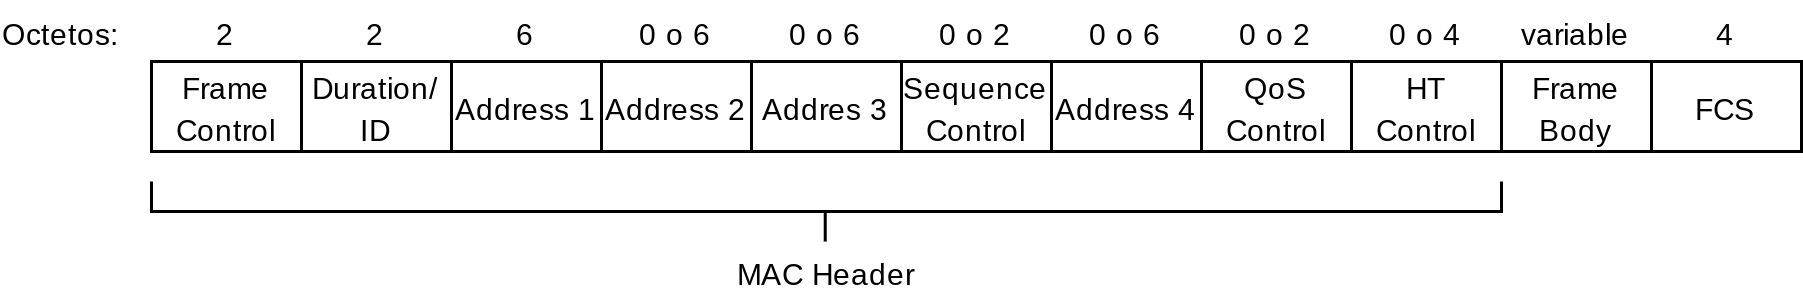
\includegraphics[scale=0.8]{analisis/mac_frame_format}
\caption{IEEE 802.11 MAC frame}
\label{fig:ieee80211_mac_frame}
\end{figure}

Los primeros tres campos (\textit{Frame Control}, \textit{Duration/ID} y \textit{Address 1}) y el último campo (\textit{FCS}) constituyen el conjunto mínimo de campos necesarios y están presentes en todas las tramas. El resto de campos están presentes solo en determinados tipos y subtipos de tramas. Para el propósito de este proyecto solo necesitamos analizar la cabecera de la trama, en concreto los campos más relevantes son el \textit{Frame Control} que permitirá determinar el tipo de trama y el campo \textit{Address 2} que almacenará la dirección MAC de la estación emisora.\\

Existen dos formatos diferentes para el campo \textit{Frame Control}, este formato viene determinado por los campos \textit{Type} y \textit{Subtype}, en este caso es de interés el formato para las tramas cuyo tipo es diferente de 1 o el subtipos es diferente de 6, en cuyo caso el campo \textit{Frame Control} será como el ilustrado en la Figura \ref{fig:ieee80211_frame_control_field}

\begin{figure}[H]
\centering
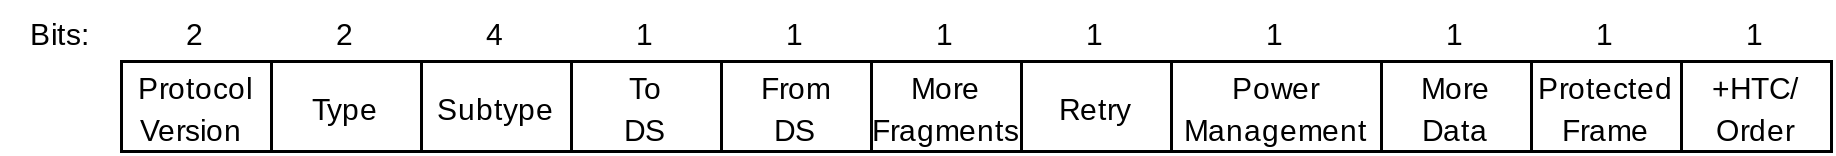
\includegraphics[scale=0.8]{analisis/frame_control_field}
\caption{IEEE 802.11 Frame Control field}
\label{fig:ieee80211_frame_control_field}
\end{figure}

El campo \textit{Type} permite determinar si se trata de una trama de tipo \textit{Management}, en la Tabla \ref{table:tipos_trama} se muestran los posibles valores que puede tomar el campo.\\

\begin{table}[h!]
\centering
\begin{tabular}{ |l|m{20em}| }
\hline
\textbf{Type} & \textbf{Descripción} \\
\hline\hline
00  & Management          \\ \hline
01  & Control  \\ \hline
10  & Data \\ \hline
11 & Extension \\ \hline
\end{tabular}
\caption{Tipos de trama IEEE 802.11}
\label{table:tipos_trama}
\end{table}

Una vez identificada la trama como tipo \textit{Management} (00) los posibles valores que puede tomar el campo \textit{Subtype} son los mostrados en la tabla \ref{table:subtipos_trama}, en concreto el valor para las tramas del subtipo \textit{Probe Request} es el 0100.

\begin{table}[h!]
\centering
\begin{tabular}{ |l|m{20em}| }
\hline
\textbf{Subtype} & \textbf{Descripción} \\
\hline\hline
0000  & Association Request  \\ \hline
0001  & Association Response \\ \hline
0010  & Reassociation Request \\ \hline
0011  & Reassociation Response \\ \hline
0100  & Probe Request \\ \hline
0101  & Probe Response \\ \hline
0110  & Timing Advertisement \\ \hline
0111  & Reserved \\ \hline
1000  & Beacon \\ \hline
1001  & ATIM \\ \hline
1010  & Disassociation \\ \hline
1011  & Authentication \\ \hline
1100  & Deauthentication \\ \hline
1101  & Action \\ \hline
1110  & Action No Ack \\ \hline
1111  & Reserved \\ \hline
\end{tabular}
\caption{Subtipos de trama para el tipo \textit{Management}}
\label{table:subtipos_trama}
\end{table}

En las tramas de tipo de tipo \textit{Management} y subtipo \textit{Probe Request} el campo \textit{Address 2} contendrá la dirección de la estación que ha emitido el \textit{Probe Request}.\\


\section{Bluetooth Low Energy}

\textit{Bluetooth Low Energy} (BLE) es una tecnología de red inalámbrica originalmente diseñada por Nokia bajo el nombre Wibree y adoptada después por el  el \textit{Bluetooth Special Interest Group}, empezó como parte de la especificación Core del Bluetooth 4.0 y fue puesta en el mercado en 2010. Desde el principio el propósito de su desarrollo fue diseñar un estándar de radio con el menor consumo posible, enfocado a dispositivos de bajo coste y con un ancho de banda bajo que no requieran realizar conexiones de larga duración ni gran volumen de tráfico de datos. A pesar del poco tiempo que lleva en el mercado ha tenido una gran adopción debido al gran crecimiento del mercado de dispositivos móviles y \textit{wearables}.\\

La capa física de BLE trabaja con 40 canales en la banda ISM de 2.4 GHz cada uno separado por 2MHz y define dos tipos de transmisiones: datos y \textit{advertising} (anuncio). 37 de estos canales se utilizan para las conexiones de datos y los últimos tres canales (37, 38 y 39) son usados como canales de \textit{advertising} para establecer nuevas conexiones o enviar datos de difusión. Se utilizan 3 canales para reducir la posibilidad de interferencia ya que estas frecuencias se comparten con otras tecnologías como el WiFi.

\begin{figure}[H]
\centering
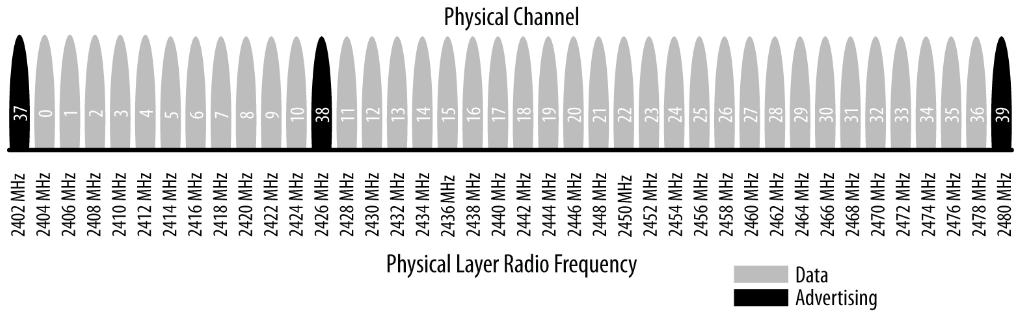
\includegraphics[scale=0.35]{analisis/ble_physical_channels}
\caption{Distribución de canales de la capa física del protocolo BLE \cite{townsend2014getting}}
\label{fig:ble_physical_channels}
\end{figure}

Para analizar en que forma podemos obtener la identificación de los dispositivos BLE es necesario analizar la capa de enlace, esta subcapa dentro la capa de Controlador define como dos dispositivos pueden transmitir información entre sí y determinados tipo de paquetes definidos en esta capa contendrán la dirección bluetooth del dispositivo emisor. La capa de enlace de BLE está definida en términos de máquinas de estado compuesta de cinco estados:  \textit{standby},  \textit{advertising},  \textit{scanning},  \textit{innitiating} y  \textit{connection}. La detección de dispositivos se da en los estados de \textit{advertising} y \textit{scanning}, cuando un dispositivo está en modo \textit{advertising} se le denomina \textit{advertiser} o anunciante, este dispositivo utiliza los tres canales de \textit{advertising} para anunciarse o enviar información, por otra parte tenemos los dispositivos en estado  \textit{scanning} denominados scanner o escáner, su propósito es permanecer a la escucha de paquetes de anuncio de anunciantes a su alrededor, pudiendo solicitarles más información. Existen también los roles maestro y esclavo utilizados cuando los dispositivos establecen una conexión bidireccional después del proceso de descubrimiento.\\

En está capa se definen dos tipos de paquetes: datos y \textit{advertising}. La principal diferencia entre estos paquetes es que los paquetes de datos solo son comprensibles para los dos dispositivos que han establecido una conexión previamente, llamados dispositivos esclavo y maestro, mientras que los paquetes de \textit{advertising} pueden estar dirigidos a un dispositivo en concreto o ser emitidos en \textit{broadcast} a cualquier dispositivo que esté escuchando, este hecho hace que este último tipo de paquetes sean de especial interés para el propósito de este proyecto, respecto al propósito de este tipo de paquetes se pueden diferenciar dos motivaciones:\\

\begin{itemize}
  \item Descubrir dispositivo esclavos y conectarse a ellos para establecer una comunicación bidireccional.
  \item Retransmitir por \textit{broadcast} datos para aplicaciones que no necesitan establecer una conexión con su consecuente sobrecarga.
\end{itemize}

Este segundo tipo de envío garantiza que un dispositivo BLE puede estar emitiendo paquetes de \textit{advertising} en cualquier momento y no solo en el proceso de descubrimiento de otros dispositivos, por ejemplo, un reloj o pulsera inteligente transmitiendo el número de pasos, esto nos permite realizar una detección de dispositivos con un menor coste computacional respecto a escanear todos los paquetes en el medio.\\

Cuando un dispositivo BLE está en modo \textit{advertising} cada paquete es enviado por los tres canales \textit{advertising} de forma secuencial, el intervalo de tiempo entre cada conjunto de estas trasmisiones está compuesto de un intervalo fijo más un intervalo aleatorio con el fin de minimizar las colisiones, el intervalo fijo se puede fijar entre 20 ms y 10.24 s y el aleatorio va desde los 0 ms hasta los 10ms, una mayor frecuencia garantiza una mayor probabilidad de que un escáner los detecte pero esto también se traduce en un mayor consumo. El ajuste de este parámetro es crucial debido al funcionamiento del proceso de descubrimiento de BLE, como se ha comentado anteriormente se utilizan tres canales para emitir con la intención de minimizar de interferencia, de esta forma el emisor se anuncia saltando entre estos tres canales y dado que este no está sincronizado con el dispositivo escáner para que un paquete de \textit{advertising} sea recibido el dispositivo anunciante y el escáner deben coincidir en el mismo canal.\\

En este proceso intervienen dos parámetros:  \textit{scan interval} y  \textit{scan window} fijados en el dispositivos escáner, estos definen cada cuanto y durante cuanto tiempo el dispositivo escáner estará escuchando. Un buen buen ajuste de estos parámetros junto al intervalo de \textit{advertising} son cruciales para incrementar la probabilidad de recepción de los paquetes sin producir un gran consumo energético.\\

\begin{figure}[H]
\centering
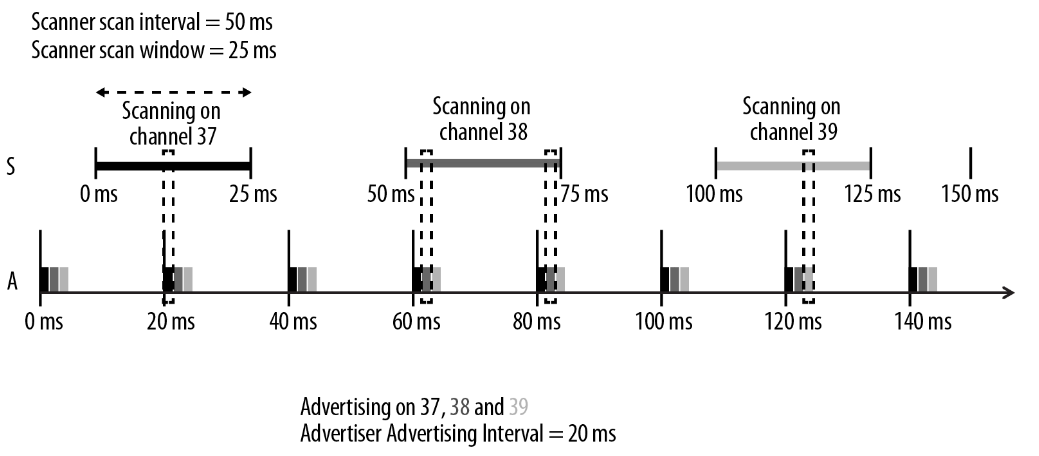
\includegraphics[scale=0.35]{analisis/ble_advertising_and_scanning}
\caption{Proceso de \textit{advertising} y escaneo en el protocolo BLE \cite{townsend2014getting}}
\label{fig:ble_advertising_and_scanning}
\end{figure}

BLE define un formato de paquete único en la capa de enlace para datos y anuncio, este paquete consta de cuatro componentes: \textit{preamble}, \textit{access address}, \textit{Protocol Data Unit} (PDU) y \textit{CRC}. El PDU es el que determinará si se trata de un paquete para el canal de datos o para el canal de anuncio, por ejemplo, los paquetes para el canal de anuncio contienen una cabecera de 16 bits y un \textit{payload} de tamaño variable que vendrá especificado en la cabecera (Figura \ref{fig:ble_advertising_pdu}). \\

\begin{figure}[H]
\centering
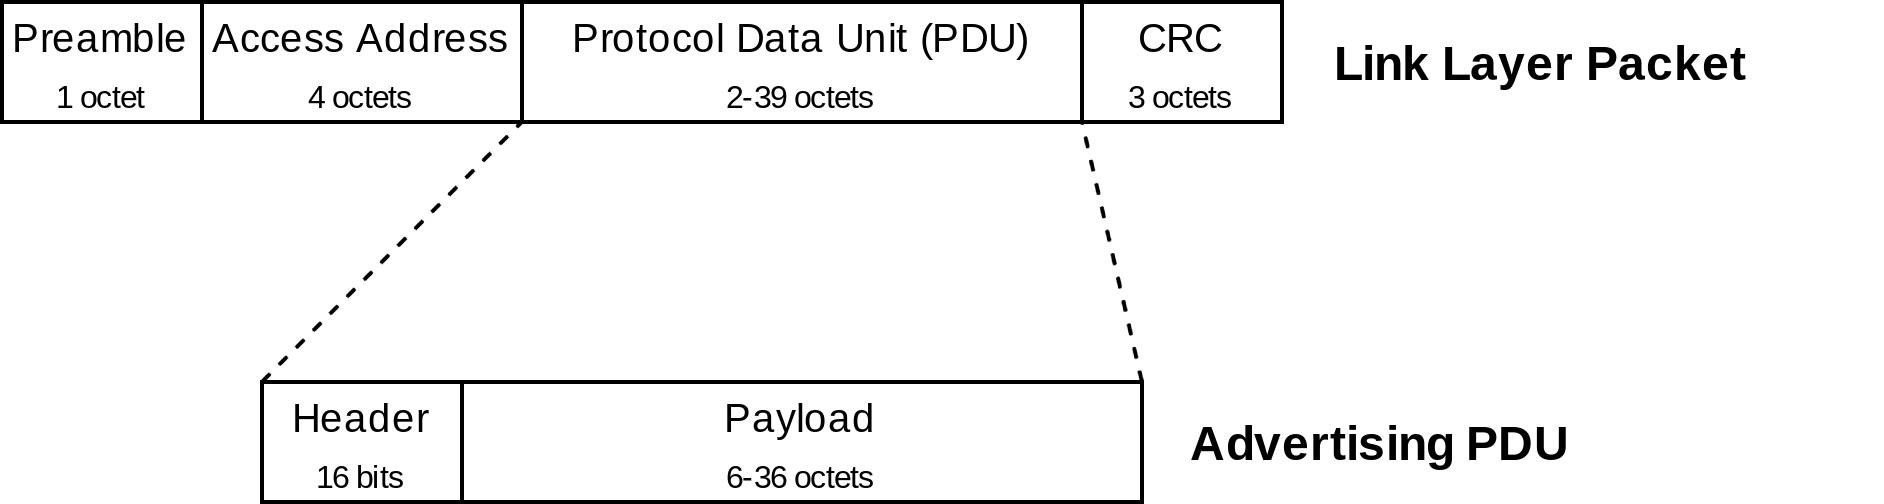
\includegraphics[scale=1]{analisis/ble_advertising_pdu}
\caption{Formato de paquete único de la capa de enlace y PDU de canal \textit{advertising}}
\label{fig:ble_advertising_pdu}
\end{figure}

La cabecera de los paquetes de canal de \textit{advertising} se componen de 6 campos (Figura \ref{fig:ble_advertaising_pdu_header}), el campo \textit{PDU Type} indica el tipo de PDU y puede tomar los valores que se muestran en la Tabla \ref{table:advertising_channel_pdu_type}. Los campos \textit{TxAdd} y \textit{TxAdd} contienen información específica dependiendo del tipo de PDU, el campo \textit{length} indica el tamaño del \textit{payload} en octetos y el campo RFU está reservado para futuros usos.\\

\begin{figure}[H]
\centering
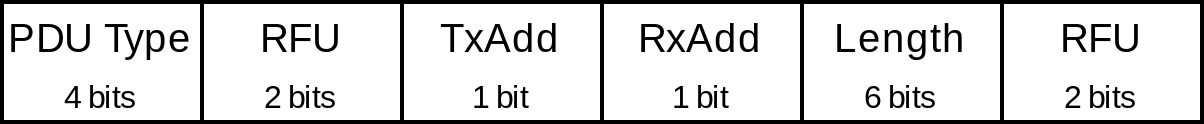
\includegraphics[scale=1]{analisis/ble_advertaising_pdu_header}
\caption{Cabecera de PDU del canal de \textit{advertising}}
\label{fig:ble_advertaising_pdu_header}
\end{figure}


\begin{table}[h!]
\centering
\begin{tabular}{ |l|m{12em}| }
\hline
\textbf{Tipo de PDU} & \textbf{Nombre de paquete} \\
\hline\hline
0000  & ADV\_IND  \\ \hline
0001  & ADV\_DIRECT\_IND  \\ \hline
0010  & ADV\_NONCONN\_IND \\ \hline
0011 & SCAN\_REQ \\ \hline
0100 & SCAN\_RSP \\ \hline
0101 & CONNECT\_REQ \\ \hline
0110 & ADV\_SCAN\_IND \\ \hline
0111-1111 & Reserved \\ \hline
\end{tabular}
\caption{Codificación para tipos de PDU definida en la cabecera de los PDUs de canal \textit{advertising}}
\label{table:advertising_channel_pdu_type}
\end{table}

Este análisis se centrará en un subconjunto de los PDUs mostrados en la Tabla \ref{table:advertising_channel_pdu_type}, los de tipo \textit{advertising}, estos son enviados por la capa de enlace en los estados de \textit{Advertising} y recibidos por la capa de enlace cuando se está en estado \textit{Scanning} o \textit{Initiating}. Este subconjunto está formado por los cuatro tipos definidos en la Tabla \ref{table:advertising_pdu_type}\\

Este tipo de PDU se pueden clasificar según tres propiedades:

\begin{itemize}
  \item Conectable: Un escáner puede iniciar una conexión tras recibir un paquete de este tipo, en caso de no poseer esta propiedad el paquete estará destinado unicamente a difusión.
  \item Escaneable: Un escáner puede emitir una solicitud de escaneo como respuesta a un paquete de este tipo solicitando más información al anunciante.
  \item Dirigido: Un paquete de este tipo está dirigido a un escáner en particular y no contiene datos de usuario en el payload solo la dirección del escáner destino, por tanto tanto los paquetes con esta propiedad son a su vez conectables.
\end{itemize}

\begin{table}[h!]
\centering
\begin{tabular}{ |l|l|l|l| }
\hline
\textbf{Tipo de PDU} & \textbf{Conectable} & \textbf{Escaneable} & \textbf{Dirigido} \\
\hline\hline
ADV\_IND  & Sí  & Sí & No \\ \hline
ADV\_DIRECT\_IND  & Sí & No & Sí \\ \hline
ADV\_NONCONN\_IND  & No & No & No \\ \hline
ADV\_SCAN\_IND &  No& Sí & No \\ \hline
\end{tabular}
\caption{Tipos de PDUs de \textit{advertising}}
\label{table:advertising_pdu_type}
\end{table}

En base a estas propiedades, resultan de interés para la detección de dispositivos los paquetes no dirigidos ya que se emiten en difusión, estos son los PDU de tipo ADV\_IND, ADV\_NONCONN\_IND y ADV\_SCAN\_IND. Los ADV\_IND son para anuncio genérico, se utilizan para anunciarse ante dispositivos centrales y que estos puedan iniciar el proceso de conexión, los ADV\_NONCONN\_IND son utilizados cuando el dispositivo anunciante no quiere establecer una conexión si no simplemente enviar información por difusión mientras que los ADV\_SCAN\_IND son utilizados para enviar información en respuesta a una solicitud de escaneo.\\

El formato del \textit{payload} de estos paquetes se describe en Figura \ref{fig:ble_advertising_pdu_payload_solo}, constan de dos campos: \textit{AdvA} y \textit{AdvData}, el primero contiene la dirección Bluetooth del anunciante y el segundo puede contener datos publicitados por el anunciante.\\

\begin{figure}[H]
\centering
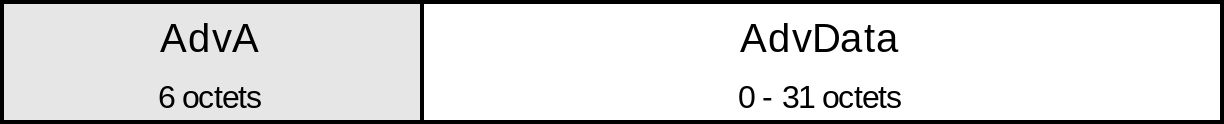
\includegraphics[scale=1]{analisis/ble_advertising_pdu_payload_solo}
\caption{Paylod del PDU de \textit{advertising}}
\label{fig:ble_advertising_pdu_payload_solo}
\end{figure}

Antes de pasar a analizar el campo \textit{AdvA} conviene realizar una breve descripción de las direcciones Bluetooth, a veces llamada dirección Bluetooth MAC y definida en el estándar como \textit{BD\_ADDR}, es un valor de 48 bits normalmente representado seis bloques de dos caracteres hexadecimales. El estándar define dos tipos de direcciones:

\begin{itemize}
  \item Pública: Es una dirección definida según el estándar EEE 802-2001 y se obtiene de la autoridad de registro del IEEE, al igual que ocurre con el estándar Ethernet esta viene fijada de fábrica y nunca cambia.
  \item Aleatoria: Esta dirección puede preprogramarse en el dispositivo (estáticas) o generarse dinámicamente (privadas) en tiempo de ejecución. Existen tres tipos: estática, privada no resoluble y privada resoluble.
\end{itemize}

Este último grupo puede generar complicaciones a la hora de rastrear un dispositivo, en el caso de las direcciones dinámicas estáticas no habría problema ya que estas pueden ser asignadas para toda la vida útil del dispositivo o en el peor de los casos regenerarse cuando el dispositivo se reinicia, sin embargo en el caso de las direcciones generadas dinámicamente puede suponer un problema dado que se regeneran continuamente, por ejemplo en el caso de los dispositivos iOS se genera una nueva cada 15 minutos, esto puede suponer un problema para el trazado de rutas de larga duración.\\

Para discernir que tipo de dirección contiene el campo \textit{AdvA} del \textit{payload} es necesario analizar el campo \textit{TxAdd} de la cabecera de este tipo de PDU que se presentaba en la Figura \ref{fig:ble_advertaising_pdu_header}, el valor de este campo permite conocer si se trata de una dirección pública (TxAdd = 0) o aleatoria (TxAdd = 1). Para este proyecto se ha decidido recoger todos los tipos de direcciones ya que aunque las direcciones aleatorias dinámicas puedan introducir algo de ruido en posible modelos generados a partir de estos datos sigue siendo de utilidad para trayectos cortos.

\section{Conclusiones}

Una vez realizado el análisis de los estándares de comunicación involucrados en los objetivos de este proyecto podemos concluir que ambos posibilitan la identificación de los dispositivos involucrados mediante una dirección de identificación única, para ello es necesario analizar el tráfico producido durante las etapas de descubrimiento y de envío de información no bidireccional en el caso del BLE, cabe destacar que la solución necesaria para su detección requiere la capacidad de poder acceder a bajo nivel a las estructuras de datos involucradas en el intercambio de información de estos protocolos.\\

\end{document}
